\documentclass[11pt]{article}

\usepackage[letterpaper, margin=1in]{geometry}
\usepackage{listings}
\usepackage[spanish]{babel}
\usepackage[utf8]{inputenc}
\usepackage{multirow}
\usepackage{tabularx}
\usepackage{longtable}
\usepackage{graphicx}



%Figuras
\usepackage{graphicx, subfigure}
\usepackage[]{tikz}
\usepackage{pbox}

%Matemática
\usepackage{amsmath}
\usepackage{amssymb}

%Símbolos mate extra (alfabetos, etc.)
\usepackage{mathrsfs}


%Algoritmos
\usepackage{float}
\usepackage{algorithm}
\usepackage{algorithmicx}
\usepackage{algpseudocode}
\usepackage{listings}


\usepackage{color}
\usepackage{hyperref}

\usepackage{mdframed}
\usepackage{tcolorbox}
\usepackage{multicol}
\usepackage{booktabs}
\usepackage{tabulary}
\definecolor{darkblue}{rgb}{0 , 0.054 , 0.196}



\title{Reporte de Laboratorio 5}
\author{Emmanuel Bustos - B51296 \\ Dunia Barahona - B40806}
\begin{document}

\maketitle
\hrule
\hrule
\tableofcontents
\hspace{5mm}
\hrule
\hrule


\section{Introducción}
Este laboratorio tuvo como propósito dotar al estudiante para adquirir habilidades en el manejo de las diferentes estructuras de datos, en específico listas, pilas y colas.
\subsection{Objetivos}
\begin{itemize}
	\item Aprender a crear e implementar listas.
	\item Aprender a crear e implementar colas.
	\item Aprender a crear e implementar pilas.
\end{itemize}

\section{Diagramas de clase}

\begin{figure}[!ht]
	\caption{Diagrama UML de la clase mazo}
	\centering
	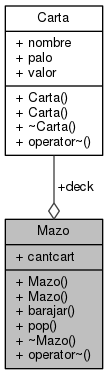
\includegraphics[width=0.16\textwidth]{1}
\end{figure}

\begin{figure}[!ht]
	\caption{Diagrama de dependencias}
	\centering
	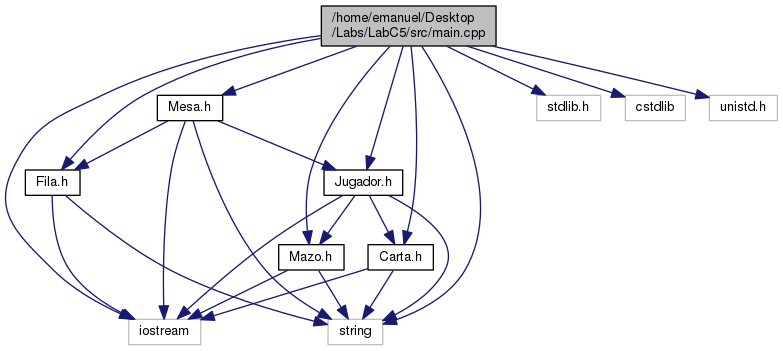
\includegraphics[width=1\textwidth]{2}
\end{figure}

\newpage

\section{Código}
\subsection{Clase fila}
\begin{lstlisting}
#include "Fila.h"
#include <iostream>
#include "string"

///Constructor basico de la clase Fila
Fila::Fila(){
}

///Constructor con caracteristicas de la clase Fila
Fila::Fila(char* fila){
this->fila = fila;
char* filo = new char[filen];
this->filord = filo;
this->D=0;
this->E=0;
this->T=0;
int i=0;
int len=0;
while(fila[i]!='\0'){
len++;
i++;
}
this->filen = len;
}

///Metodo de la clase fila que crea salas de espera en las cuales agrupa a su contenido segun su tipo
void Fila::salas(){
int i=0;
int t=0;
while(i<filen){
if(fila[i]=='T'){
t++;
}
if(fila[i]=='E'){
this->E++;
}
if(fila[i]=='D'){
this->D++;
}
i++;
}
this->T=t;
}

///Metodo que ordena la fila segun la prioridad
void Fila::ord(){
this->salas();
D=this->D;
T=this->T;
E=this->E;
float i=0;
float j=0;
float k=0;
int cont=filen-1;
while(D!=0 || T!=0 || E!=0){
i+=2;
j+=1;
k+=0.5;
if(i==2 && E!=0){
filord[cont]= 'E';
E--;
cont--;
i=0;
}
if(j==2 && T!=0){
filord[cont]= 'T';
T--;
cont--;
j=0;
}
if(k==2 && D!=0){
filord[cont]= 'D';
D--;
cont--;
k=0;
}
}
}

///Metodo que extrae el ultimo elemento de la cola fila ordenada
char Fila::pop(bool cond){
if(cond && filen!=0){
this->filen--;
return this->filord[filen];
}
}

///Destructor de la clase Fila
Fila::~Fila(){
}

///Metodo de impresion para la clase Fila
void Fila::operator~(){
for(int i=0;i<this->filen;i++){
cout<<this->filord[i]<< ' ';
}
cout<<endl;
}
\end{lstlisting}

\subsection{Clase Mazo}
\begin{lstlisting}
#include "Carta.h"
#include <iostream>
#include "string"
#include "Mazo.h"
#include <cstdlib>
#include "time.h"
///Constructor basico de clase Mazo
Mazo::Mazo(){
this->cantcart=52;
this->deck = new Carta[52];
this->deck[0]=Carta("As", "Picas", 11);
this->deck[1]=Carta("Dos", "Picas", 2);
this->deck[2]=Carta("Tres", "Picas", 3);
this->deck[3]=Carta("Cuatro", "Picas", 4);
this->deck[4]=Carta("Cinco", "Picas", 5);
this->deck[5]=Carta("Seis", "Picas", 6);
this->deck[6]=Carta("Siete", "Picas", 7);
this->deck[7]=Carta("Ocho", "Picas", 8);
this->deck[8]=Carta("Nueve", "Picas", 9);
this->deck[9]=Carta("Diez", "Picas", 10);
this->deck[10]=Carta("J", "Picas", 10);
this->deck[11]=Carta("Q", "Picas", 10);
this->deck[12]=Carta("K", "Picas", 10);

this->deck[13]=Carta("As", "Diamantes", 11);
this->deck[14]=Carta("Dos", "Diamantes", 2);
this->deck[15]=Carta("Tres", "Diamantes", 3);
this->deck[16]=Carta("Cuatro", "Diamantes", 4);
this->deck[17]=Carta("Cinco", "Diamantes", 5);
this->deck[18]=Carta("Seis", "Diamantes", 6);
this->deck[19]=Carta("Siente", "Diamantes", 7);
this->deck[20]=Carta("Ocho", "Diamantes", 8);
this->deck[21]=Carta("Nueve", "Diamantes", 9);
this->deck[22]=Carta("Diez", "Diamantes", 10);
this->deck[23]=Carta("J", "Diamantes", 10);
this->deck[24]=Carta("Q", "Diamantes", 10);
this->deck[25]=Carta("K", "Diamantes", 10);

this->deck[26]=Carta("As", "Corazones", 11);
this->deck[27]=Carta("Dos", "Corazones", 2);
this->deck[28]=Carta("Tres", "Corazones", 3);
this->deck[29]=Carta("Cuatro", "Corazones", 4);
this->deck[30]=Carta("Cinco", "Corazones", 5);
this->deck[31]=Carta("Seis", "Corazones", 6);
this->deck[32]=Carta("Siete", "Corazones", 7);
this->deck[33]=Carta("Ocho", "Corazones", 8);
this->deck[34]=Carta("Nueve", "Corazones", 9);
this->deck[35]=Carta("Diez", "Corazones", 10);
this->deck[36]=Carta("J", "Corazones", 10);
this->deck[37]=Carta("Q", "Corazones", 10);
this->deck[38]=Carta("K", "Corazones", 10);

this->deck[39]=Carta("As", "Trebol", 11);
this->deck[40]=Carta("Dos", "Trebol", 2);
this->deck[41]=Carta("Tres", "Trebol", 3);
this->deck[42]=Carta("Cuatro", "Trebol", 4);
this->deck[43]=Carta("Cinco", "Trebol", 5);
this->deck[44]=Carta("Seis", "Trebol", 6);
this->deck[45]=Carta("Siete", "Trebol", 7);
this->deck[46]=Carta("Ocho", "Trebol", 8);
this->deck[47]=Carta("Nueve", "Trebol", 9);
this->deck[48]=Carta("Diez", "Trebol", 10);
this->deck[49]=Carta("J", "Trebol", 10);
this->deck[50]=Carta("Q", "Trebol", 10);
this->deck[51]=Carta("K", "Trebol", 10);

}

///Destructor de la clase mazo
Mazo::~Mazo(){
}

///Metodo que de forma aleatoria ordena a las cartas del objeto mazo
void Mazo::barajar(){
srand(time(0));
Carta cartemp;
int m;
int n;
for(int i=0; i<300; i++){
m=rand()%(cantcart);
n=rand()%(cantcart);
cartemp=this->deck[m];
this->deck[m]=this->deck[n];
this->deck[n]=cartemp;
}
}

///Metodo que hace un pop al mazo, removiendo la carta que esta arriba en el strack
Carta Mazo::pop(bool cond){
if(cond && cantcart!=0){
this->cantcart--;
return this->deck[cantcart];
}
}

///Metodo de print para la clase mazo
void Mazo::operator~(){
for(int i=0; i<cantcart; i++){
~deck[i];
}
}

\end{lstlisting}

\subsection{Clase Carta}
\begin{lstlisting}
#include "Carta.h"
#include <iostream>
#include "string"
///Constructor basico de la clase Carta
Carta::Carta(){
}

///Constructor con caracteristicas de la clase Carta
Carta::Carta(string nombre, string palo, int valor){
this->nombre = nombre;
this->palo=palo;
this->valor=valor;
}

///Destructor de la clase Carta
Carta::~Carta(){
}

///Metodo de print para la clase Carta
void Carta::operator~(){
cout<< this->nombre << " de " << this->palo << " con valor de " << this->valor << endl;
}
\end{lstlisting}

\subsection{Clase Jugador}
\begin{lstlisting}
#include "Jugador.h"
#include <iostream>
#include "string"
#include "Carta.h"
#include "Mazo.h"
///Constructor basico de la clase Jugador
Jugador::Jugador(){
}
///Constructor con caracteristicas de la clase Jugador
Jugador::Jugador(int n){
this->puntos=0;
this->activo=false;
this->numero=n;
}

///Destructor de la clase Jugador
Jugador::~Jugador(){
}

///Metodo de print para objetos Jugador
void Jugador::operator~(){
cout<<"El jugador "<<numero<< " posee "<< puntos<<" puntos"<<endl;
}

///Metodo de la clase jugador para comer carta de un mazo
void Jugador::comer(Mazo &mazo){
Carta carta=mazo.pop(true);
this->puntos+=carta.valor;
}
\end{lstlisting}

\subsection{Main}
\begin{lstlisting}
#include <iostream>
#include "string"
#include "Fila.h"
#include "Carta.h"
#include "Mazo.h"
#include "Jugador.h"
#include "Mesa.h"
#include "stdlib.h"   
#include <cstdlib>
#include <unistd.h>
using namespace std;
int main(int argc, char** argv) {
Fila A= Fila(argv[1]);
A.ord();
cout<< A.T <<endl;
Mesa Mesa1(1);
Mesa Mesa2(2);
Mesa Mesa3(3);
while(A.filen!=0){
Mesa1.partida(A);
usleep(1000000); //Delay agregado para evitar errores con la semilla de funcion random
Mesa2.partida(A);
usleep(1000000);
Mesa3.partida(A);
usleep(1000000);
}

while(Mesa1.espaciosdisp!=3){
Mesa1.partida(A);
usleep(1000000);
}

while(Mesa2.espaciosdisp!=3){
Mesa2.partida(A);
usleep(1000000);
}

while(Mesa3.espaciosdisp!=3){
Mesa3.partida(A);
usleep(1000000);
}

if(Mesa1.espaciosdisp==3 && Mesa1.espaciosdisp==3 && Mesa1.espaciosdisp==3 && A.filen==0){
cout<<"Casino vacio"<<endl;
}

return 0;
}

\end{lstlisting}

\section{Conclusiones}
Con ayuda de este laboratorio, se desarrollaron las habilidades para manejar las listas, pilas y colas, estructuras de datos realmente útiles para manejar y organizar diferentes tipos de datos.




\end{document}
